\input templates/header
\title[DS - Reliable Broadcast]{\textbf{Distributed Algorithms}\\Reliable Broadcast}



\begin{document}

\FrameTitle
\FrameContent

\section{Introduction}

\begin{frame}{Introduction}

Efficient techniques are required, capable of supporting consistent behavior 
between system components in spite of failures.

\bigskip
\begin{block}{Examples}
\BIL
\item  \alert{Reliable Broadcast/Multicast protocols}:\\
Ensure reliable message delivery to all participants 
\item Agreement protocols:\\
Ensure all participants to have a consistent system view 
\item Commit protocols:\\
Implement atomic behavior in transactional types of systems
\EIL
\end{block}

\end{frame}

\begin{frame}{Broadcast}
	
\begin{figure}
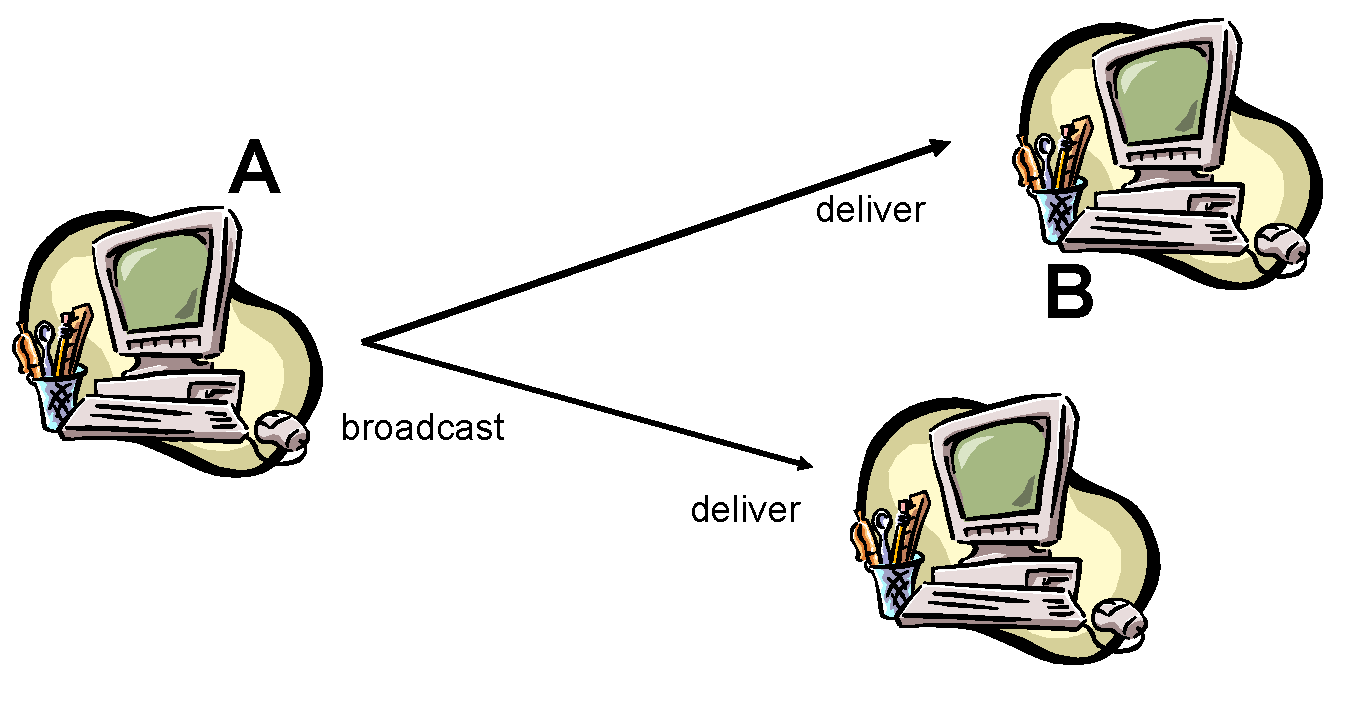
\includegraphics[width=\textwidth]{figs/04/rb-example}
\end{figure}

\end{frame}

\begin{frame}{Broadcast Protocol Layering}
	
\begin{figure}
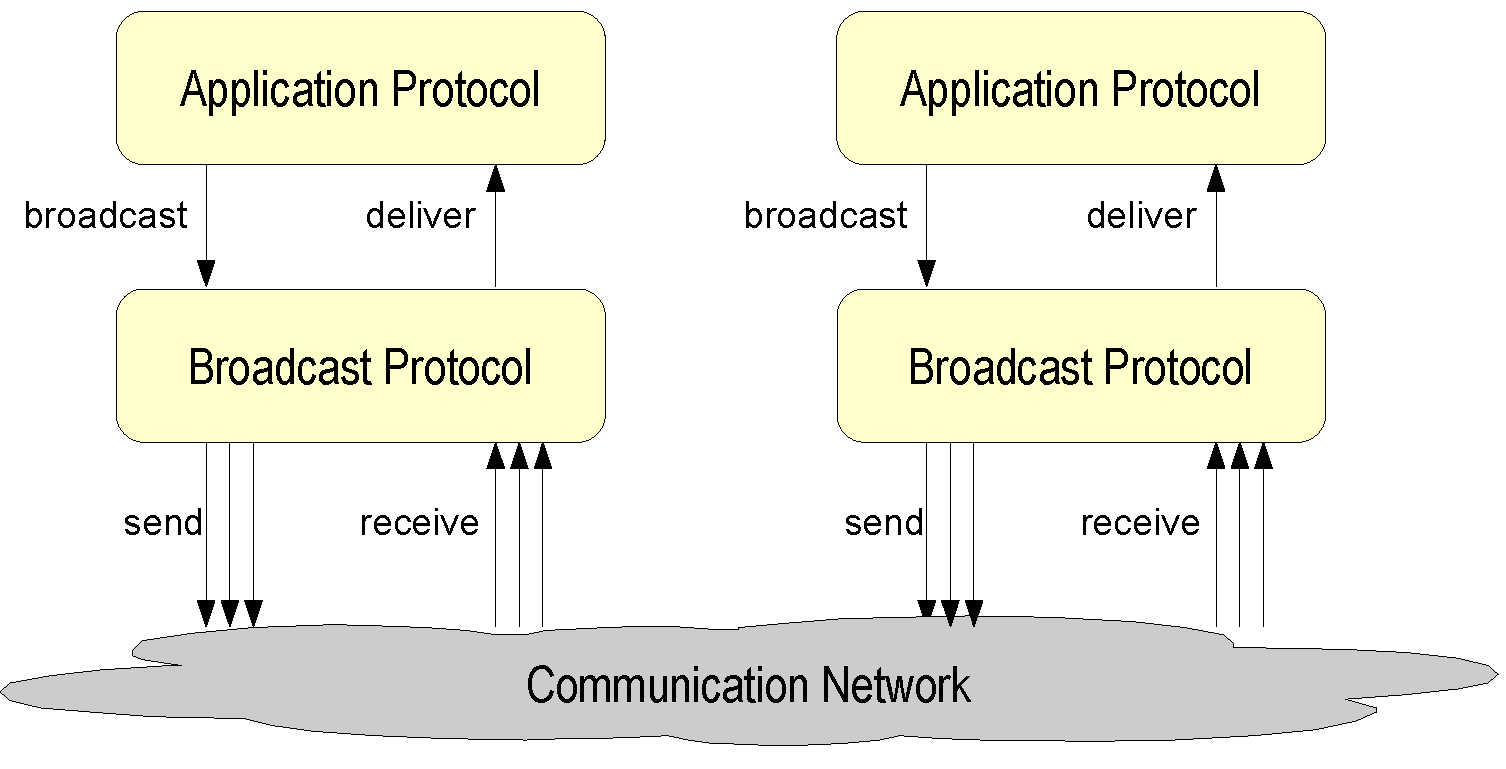
\includegraphics[width=\textwidth]{figs/04/layers}
\end{figure}

\end{frame}


\begin{frame}{Basic assumptions (1)}
	
\BIL

\item \alert{System is asynchronous}
	\BI
	\item No bounds on messages and process execution delays
	\EI
	
\item \alert{Processes fail by crashing}
	\BI
	\item stop executing actions after the crash
	\item We do not consider Byzantine failures
	\EI
	
\item \alert{Correct/Faulty}
	\BI
	\item A process that does not fail in a run is \alert{correct} in that run
	\item Otherwise, the process is \alert{faulty}
	\EI
	
\EIL

\end{frame}

\begin{frame}{Basic assumptions (2)}
	
We will consider two failure models for communication:

\bigskip
\begin{block}{No Failures}
\BIL
\item \alert{Validity}: If $p$ sends a message to $q$, and $q$ is correct, then $q$ will eventually receive $m$
\item \alert{Integrity}: No message is delivered to a process more than once, and only if it has been sent previously
\EIL
\end{block}

\bigskip
\begin{block}{Perfect Channels}
\BIL
\item \alert{Validity}: If $p$ sends a message to $q$, and $p$,$q$ are correct, then $q$ will eventually receive $m$
\item \alert{Integrity}: No message is delivered to a process more than once, and only if it has been sent previously
\EIL
\end{block}

\end{frame}

\begin{frame}{What kind of underlying network?}

\BIL

\item \alert{Complete graph}
\BI
\item Every process can communicate with every other process
\item A routing substrate realizes this abstraction
\EI

\item \alert{Point-to-point}
\BI
\item Every process can communicate with a subset of processes 
(its neighbors)
\item Routing is not implemented at the send/receive level 
(we may implement it at the level of our protocols)
\EI

\EIL

\end{frame}

\begin{frame}{Different flavors of broadcast}
	
\begin{columns}[t]
\begin{column}{0.5\textwidth}
\BIL

\item Reliability
\BI
\item \textbf{B}est-effort 
\item \textbf{R}eliable 
\item \textbf{U}niform \textbf{R}eliable 
\EI

\item Ordering

\BI
\item \textbf{F}IFO
\item \textbf{C}asual
\item \textbf{A}tomic
\item \textbf{F}IFO \textbf{A}tomic
\item \textbf{Causal} \textbf{A}tomic
\EI

\EIL
\end{column}
\begin{column}{0.5\textwidth}

\BIL 

\item Time bounds
\BI
\item \textbf{T}imed \textbf{R}eliable 
\EI

\item Primitives
\BI
\item R-Broadcast
\item F-Broadcast
\item C-Broadcast
\item \ldots
\EI

\EIL
\end{column}
\end{columns}

\end{frame}

\section{Broadcast specifications and protocols}

\subsection{Best-Effort Broadcast}

\begin{frame}{Best-effort broadcast -- Specification}

\begin{definition}[BEB1 -- Validity]
If $p$ and $q$ are correct, then every message B-broadcast by $p$ is eventually delivered by $q$
\end{definition}

\begin{definition}[BEB2 -- Uniform Integrity]
$m$ is delivered by a process at most once, and only if it was previously broadcast
\end{definition}

\end{frame}

\begin{frame}{Best-effort broadcast -- Algorithm}

\begin{Procedure}
\caption{Best-effort broadcast protocol executed by $p$}

\UPON{$\bbroadcast(m)$}{
  \ForEach{$q \in \Pi$}{
    \SEND $m$ \TO $q$\;
  }
}
\BlankLine
\UPON{$\RECEIVE(m)$}{
  $\bdeliver(m)$\;
}

\end{Procedure}

\begin{block}{Notation -- Send to all}
\RestyleAlgo{plain}
	
\begin{minipage}{4cm}
\begin{Procedure}
\ForEach{$q \in \Pi$}{
  \SEND $m$ \TO $q$\;
}
\end{Procedure}
\end{minipage}
\quad is equivalent to \quad
\begin{minipage}{4cm}
\begin{Procedure}
\SEND $m$ \TO $\Pi$\;
\end{Procedure}
\end{minipage}
\RestyleAlgo{ruled}

\end{block}


\end{frame}

\begin{frame}{Best-effort broadcast -- Proof}

\structure{We can show that the protocol works with \emph{Perfect Channels}}:

\BIL
\item \alert{BEB1 - Validity}: By the Validity property of Perfect Channels and the very facts that 
\BE
\item the sender sends the message to all 
\item every correct process that receives a message B-delivers it
\EE
\item \alert{BEB2 -- Uniform Integrity}: By the Integrity property of Perfect Channels
\EIL

\bigskip
\structure{Clearly, it will work also with No Failures}

\end{frame}

\begin{frame}{Best-effort broadcast -- Example}
	
\begin{figure}
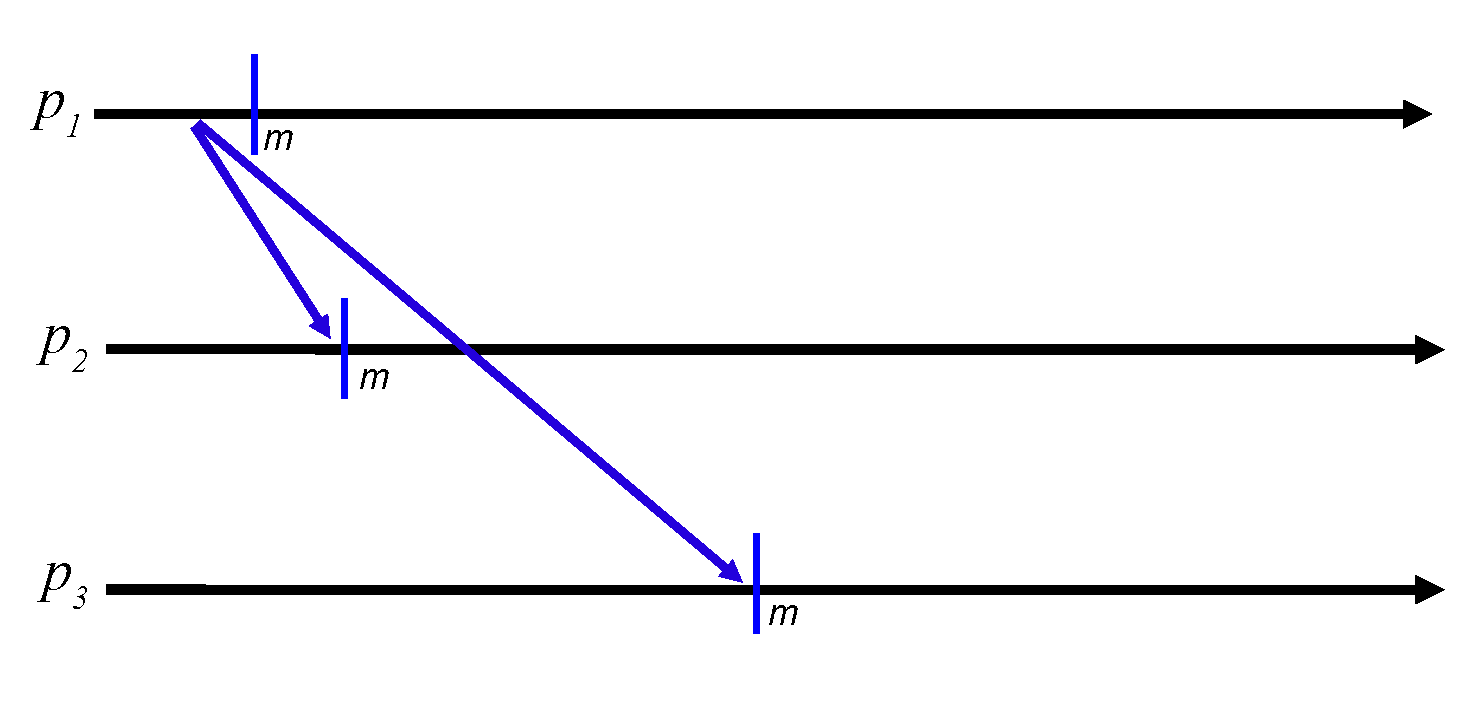
\includegraphics[width=\textwidth]{figs/04/beb-normal}
\end{figure}

\end{frame}

\begin{frame}{Best-effort broadcast -- Example}
	
\begin{figure}
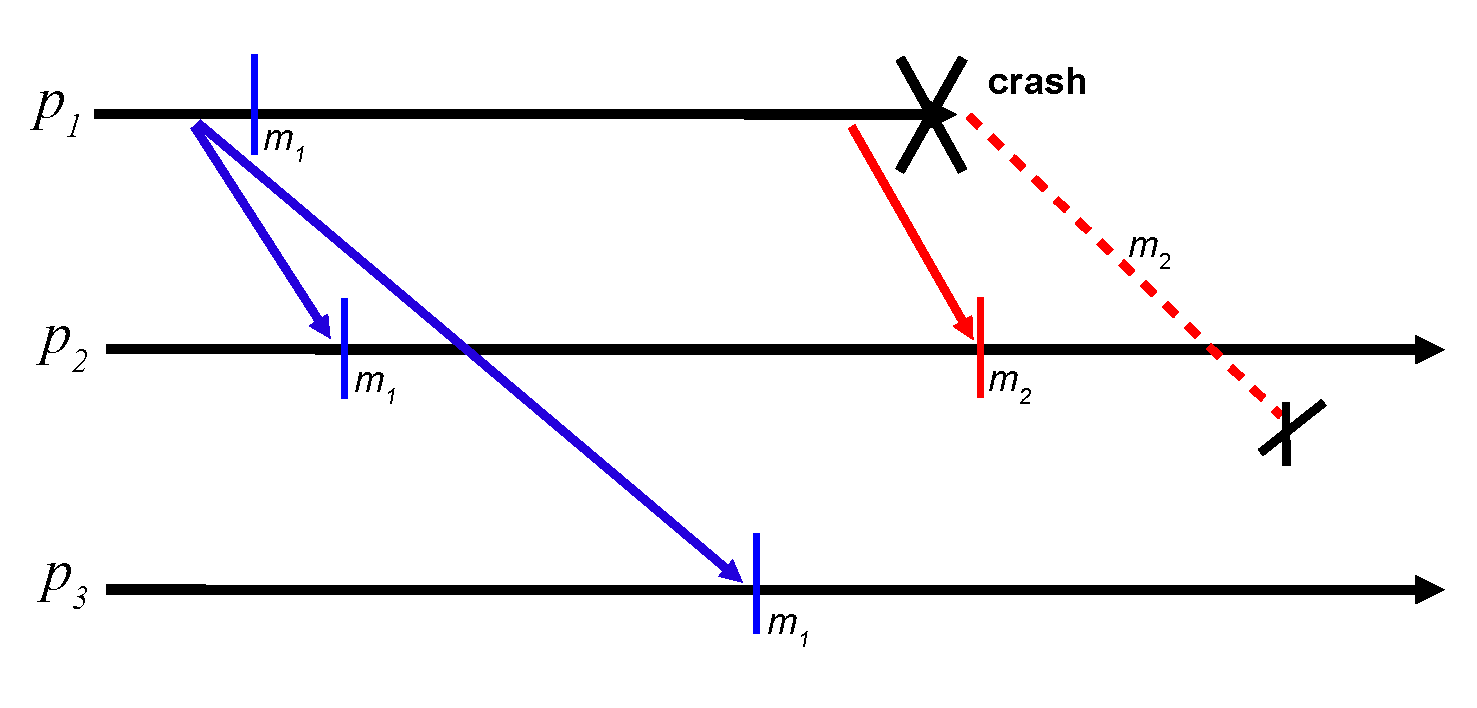
\includegraphics[width=\textwidth]{figs/04/beb-failure}
\end{figure}

\end{frame}

\begin{frame}{Best-effort broadcast -- Problem}
	
\structure{What happens if the sender fails?}

\BIL
\item Even in the absence of communication failures:
\BI
\item if the sender crashes before being able to send  the message to all
\item some processes will not deliver the message
\EI
\EIL

\bigskip
\structure{What we do?}

\BIL
\item First we revise the specification of broadcast
\item Then we implement the new specification	
\EIL

\end{frame}

\subsection{Reliable Broadcast}

\begin{frame}{Reliable Broadcast -- Specification}

\begin{definition}[RB1 -- Validity]
If a correct process broadcasts $m$, then it eventually delivers $m$
\end{definition}

\begin{definition}[RB2 -- Uniform Integrity]
$m$ is delivered by a process at most once, and only if 
it was previously broadcast
\end{definition}

\begin{definition}[RB3 -- Agreement]
If a correct process delivers $m$, then all correct processes eventually deliver $m$
\end{definition}



\end{frame}

\begin{frame}{Reliable Broadcast -- Scenario 1}

\structure{Does this execution satisfy the RB specification?}

\begin{figure}
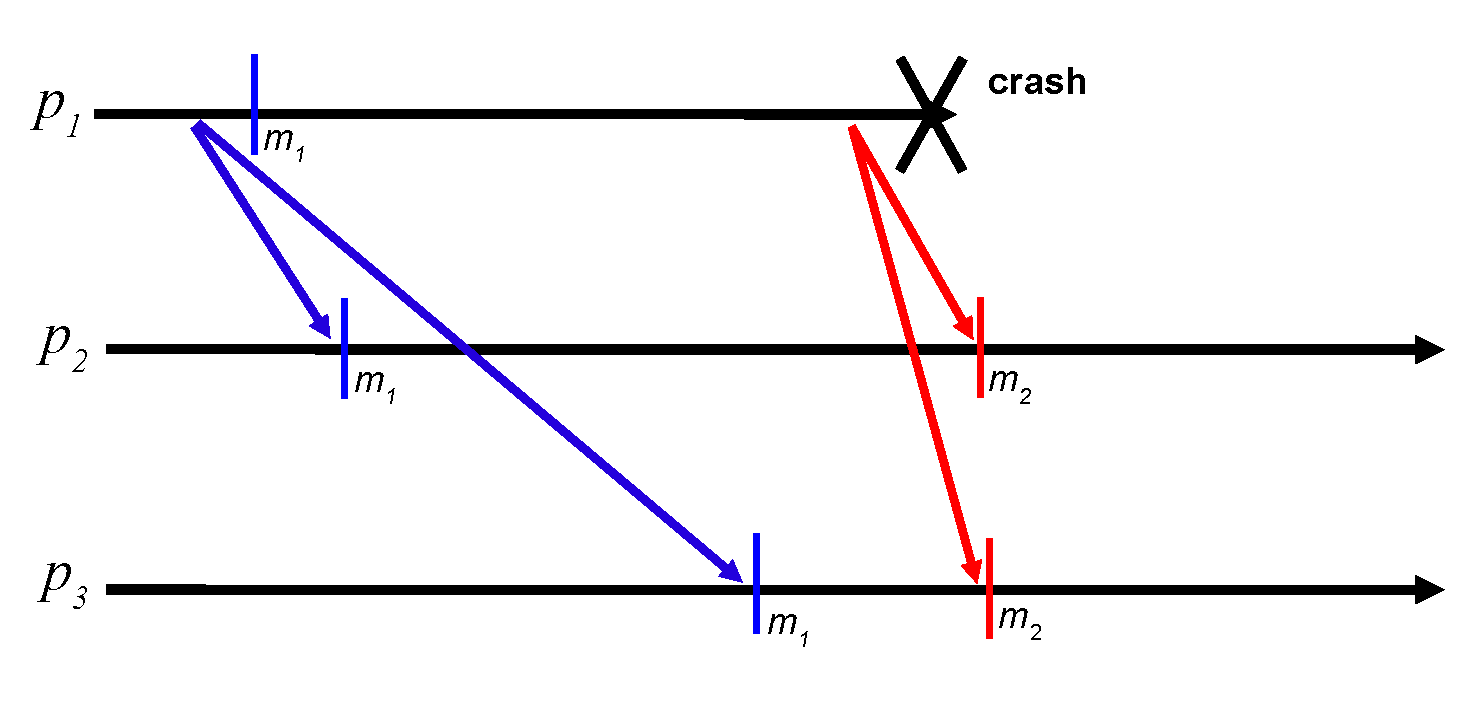
\includegraphics[width=\textwidth]{figs/04/rb-scenario1}
\end{figure}

\note{
  Obviously yes -- the fact that process $p_1$ does not deliver $m$ is not
a problem, because Validity only requires correct processes to deliver their
own messages.
}


\end{frame}

\begin{frame}{Reliable Broadcast -- Scenario 2}

\structure{Does this execution satisfy the RB specification?}

\begin{figure}
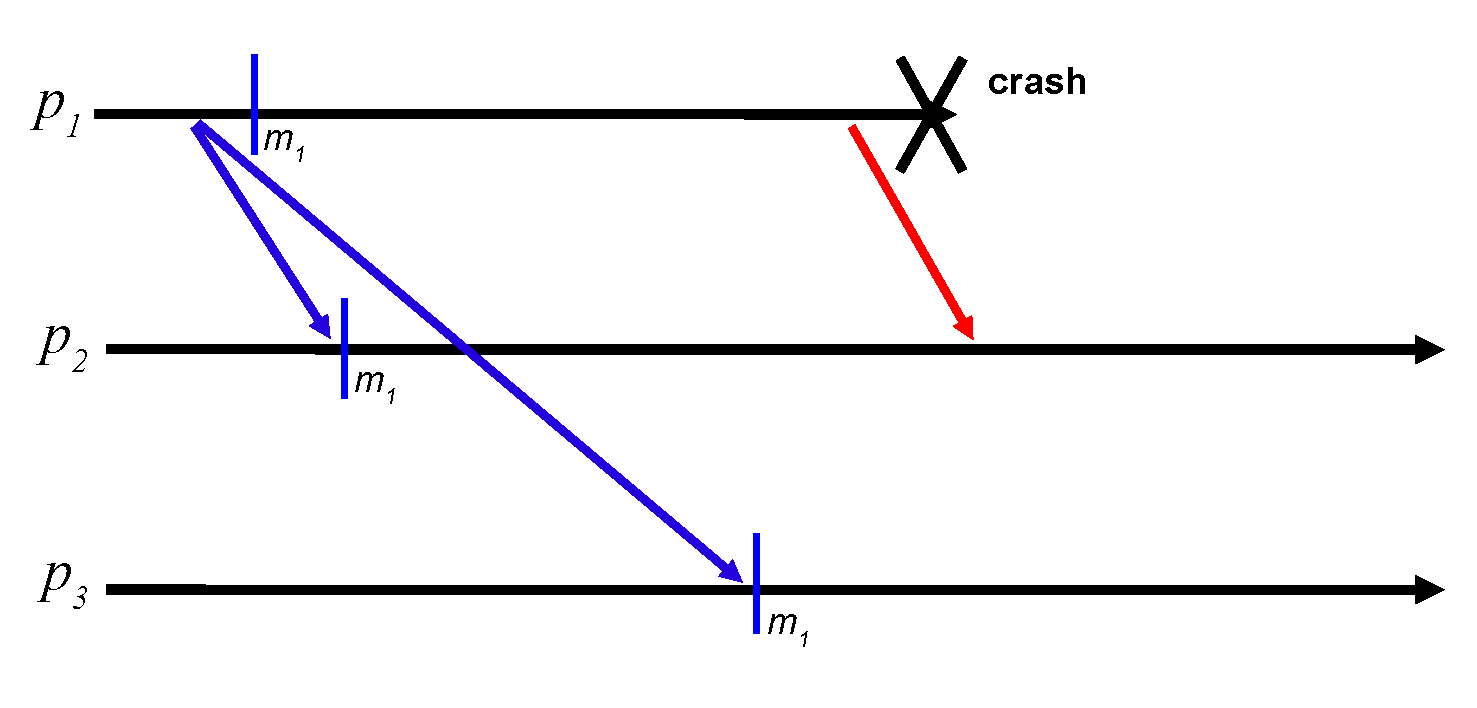
\includegraphics[width=\textwidth]{figs/04/rb-scenario2}
\end{figure}

\note{Obviously yes -- the fact that no process delivers $m$ is not a 
problem, because process $p_1$ is faulty and Validity does not apply;
and nobody delivers $m$, so Agreement does not apply.}

\end{frame}

\begin{frame}{Reliable Broadcast -- Scenario 3}

\structure{Does this execution satisfy the RB specification?}

\begin{figure}
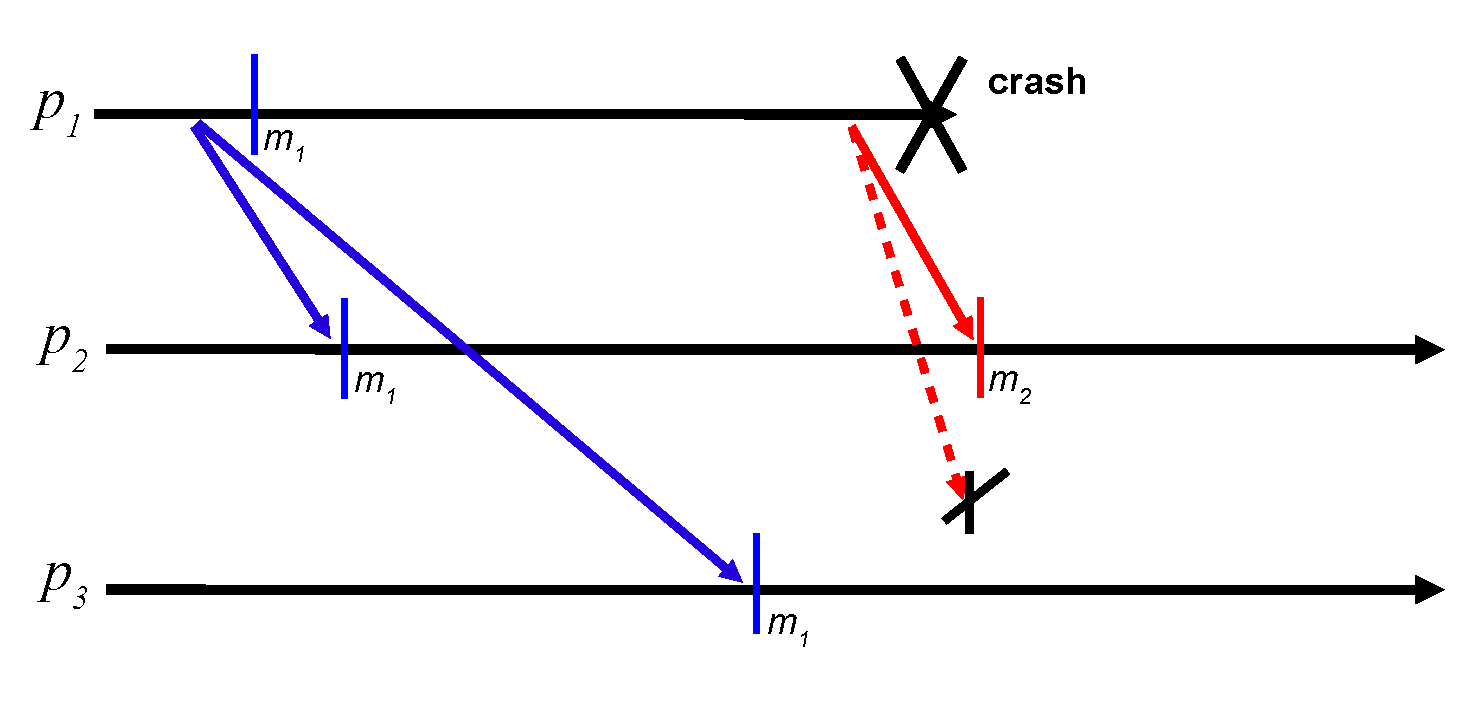
\includegraphics[width=\textwidth]{figs/04/rb-scenario3}
\end{figure}

\note{Obviously no -- Agreement is not satisfied.}

\end{frame}

\begin{frame}{Reliable Broadcast -- Algorithm v.1}



\begin{Procedure}
\caption{Reliable broadcast protocol executed by $p$}
\UPON{initialization}{
	$\Set\ \Delivered \gets \emptyset$\Comment*[f]{Messages already delivered}\;
}
\BlankLine
\UPON{$\rbroadcast(m)$}{
  \SEND $m$ \TO $\Pi - \{p\}$\;
  $\rdeliver(m)$\;
  $\Delivered \gets \Delivered \cup \{ m \}$\;
} 
\BlankLine
\UPON{$\RECEIVE(m)$ \From $q$}{
  \If{\NOT $m \in \Delivered$}{
    \SEND $m$ \TO $\Pi-\{ p, q \}$\;
    $\rdeliver(m)$\;
    $\Delivered \gets \Delivered \cup \{ m \}$\;
  }
}

\end{Procedure}

\end{frame}

\begin{frame}{Reliable Broadcast -- Scenario 4}

\structure{Does this execution satisfy the RB specification?}

\begin{figure}
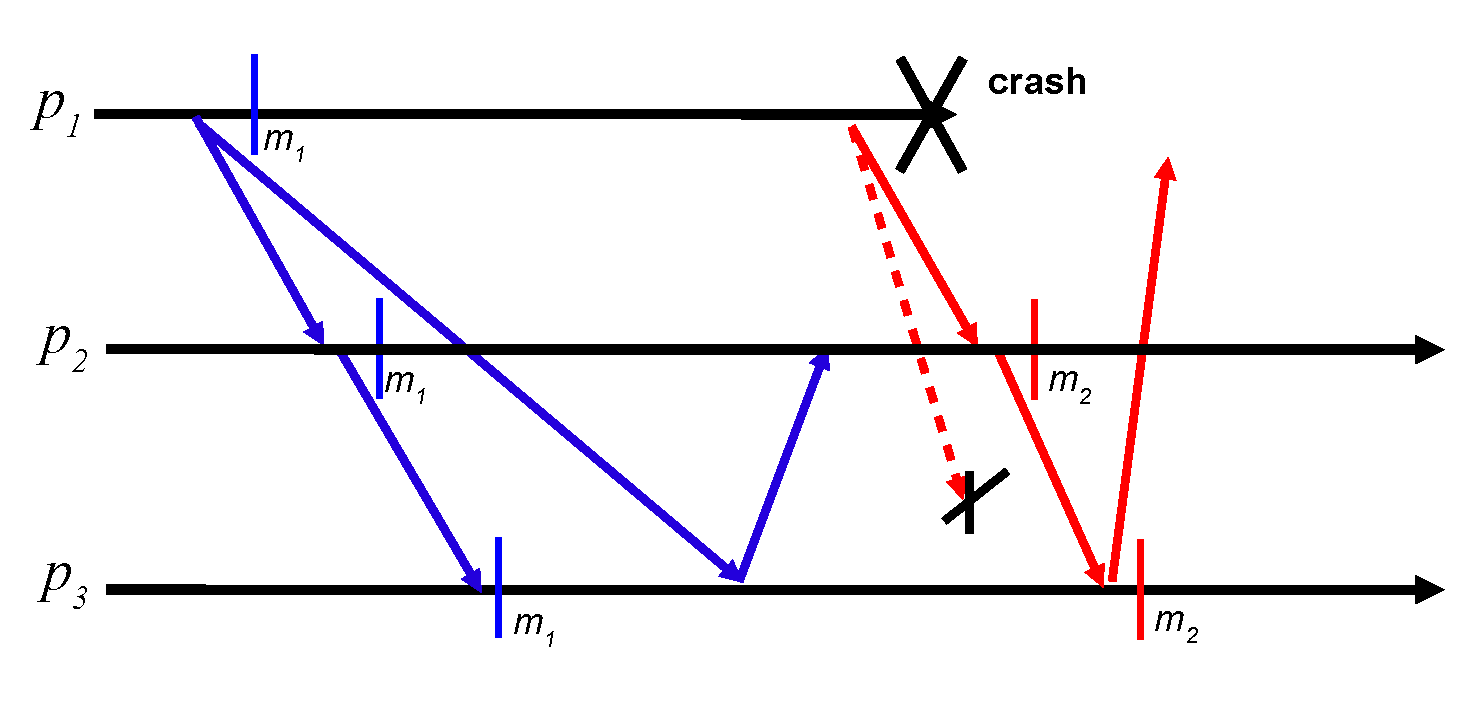
\includegraphics[width=\textwidth]{figs/04/rb-correct-scenario}
\end{figure}

\note{Yes, because before R-delivering the message, $p_2$ forwards it
to all other processes.}

\end{frame}



\begin{frame}{Reliable Broadcast -- Proof}

\structure{Algorithm v.1 implements Reliable Broadcast.}

\BIL
\item \alert{RB1 -- Validity}: \emph{If a correct process broadcasts $m$, then it eventually delivers $m$}\\
By the code implementing R-broadcast.
\item \alert{RB2 -- Agreement}: \emph{If a correct process delivers $m$, then all correct processes eventually deliver $m$}\\
Before R-delivering $m$, a correct process $p$ forwards $m$ to all processes. 
By Validity of Perfect Channels and the fact that $p$ is correct, all correct processes will eventually receive $m$ and R-deliver it.
\item \alert{RB3 -- Integrity}: \emph{$m$ is delivered by a process at most once, and only if it was previously broadcast}\\
By the Integrity of Perfect Channels and the use of variable $\Delivered$
\EIL

\end{frame}

\begin{frame}{Reliable Broadcast -- Scenario 5}

\structure{Does this execution satisfy the RB specification?}

\begin{figure}
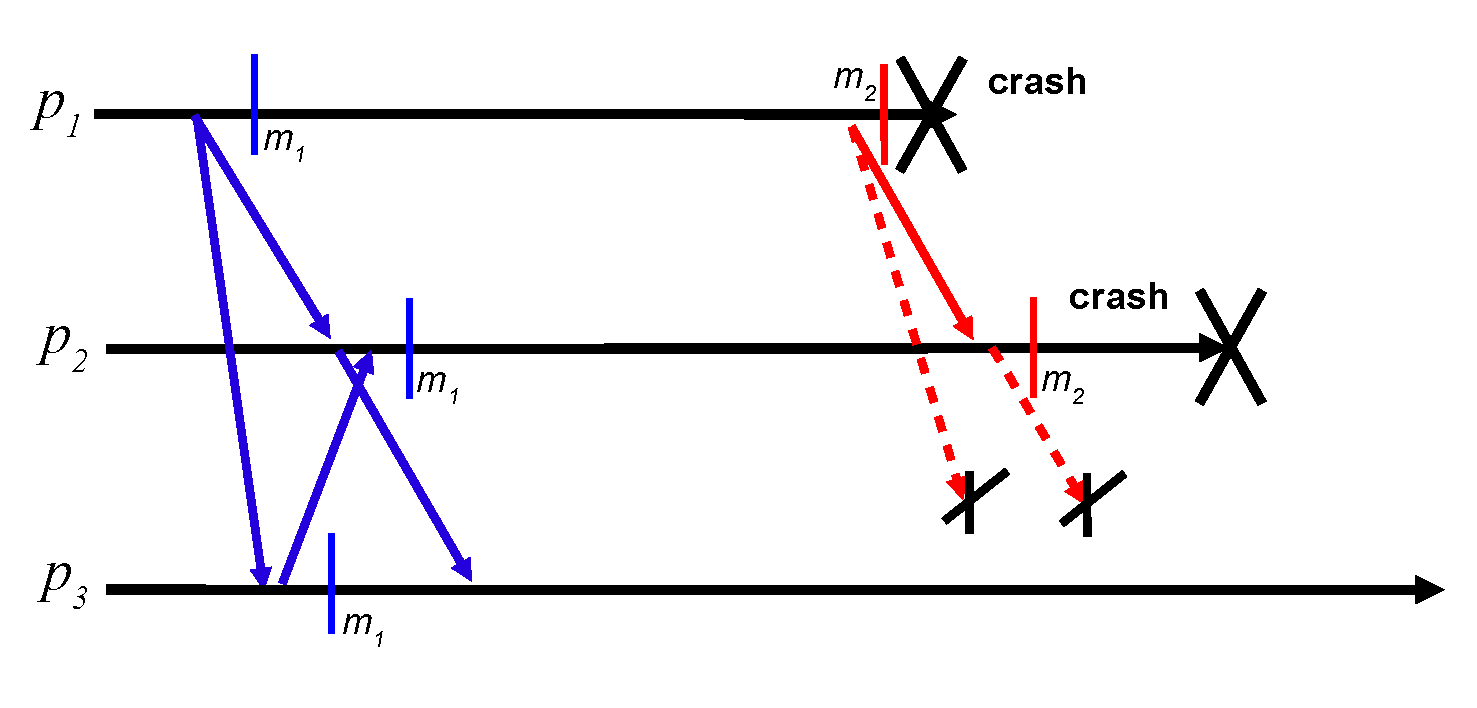
\includegraphics[width=\textwidth]{figs/04/rb-scenario5}
\end{figure}

\note{Yes, because the fact that $m_1$ has been delivered by $p_1$ 
and $p_2$, which are not correct, does not imply that $m_1$ has to
be delivered by $p_3$ as well. Yet, this situation is not desirable,
because two processes deliver something and another one does not.}

\end{frame}

\subsection{Uniform Reliable Broadcast}

\begin{frame}{Uniform Reliable Broadcast -- Specification}

\begin{definition}[URB1 -- Validity]
If a correct process broadcasts $m$, then it eventually delivers $m$
\end{definition}

\begin{definition}[\alert{URB2 -- Uniform Agreement}]
If a \sout{correct} process delivers $m$, then all correct processes eventually deliver $m$
\end{definition}

\begin{definition}[URB3 --- Uniform Integrity]
$m$ is delivered by a process at most once, and only if 
it was previously broadcast
\end{definition}

\end{frame}

\begin{frame}{Uniform Reliable Broadcast -- Proof}

\structure{Algorithm v.1 implements Uniform Reliable Broadcast...}

\structure{... but under different assumptions!}



\BIL
\item \textbf{URB1}, \textbf{URB2}: As \textbf{RB1}, \textbf{RB2}
\item \textbf{RB3 -- Uniform Agreement}: If a process delivers $m$, then all correct processes eventually deliver $m$
\BI
\item Before R-delivering $m$, a process forwards $m$ to all processes. 
\item \sout{By Validity of Perfect Channels, all correct processes will eventually receive $m$ and R-deliver it}
\item In the \alert{absence of communication failures}, all correct processes will eventually receive $m$ and R-deliver it
\EI
\EIL

\end{frame}

%%%%%%%%%%%%%%%%%%%%%%%%%%%%%%%%%%%%%%%%%%%%%%%%%%%%%%%%%%%%%%%%%%%%%%%%

\addtocontents{toc}{\newpage}

\section{Message ordering}

\subsection{Introduction}

\begin{frame}{Message ordering}

\begin{block}{Problem}
\BI
\item Given the asynchronous nature of distributed systems, messages may be delivered	
in any order
\item Some services, such as replication, need messages to be delivered in a
consistent manner, otherwise replicas may diverge.
\EI
\end{block}

\bigskip
\begin{block}{Solution}
We describe a collection of ordering policies and we show how to 
implement them in a modular way.
\end{block}

\end{frame}

\subsection{Specification}

\begin{frame}{Message ordering}

\begin{definition}[FIFO Order]
If a process $p$ broadcasts a message $m$ before it broadcast a message $m'$, the 
no correct process delivers $m'$ unless it has previously delivered $m$
\[
  \broadcast_p(m) \rightarrow \broadcast_p(m') \Rightarrow \deliver_q(m) \rightarrow \deliver_q(m')
\]
\end{definition}
		
\end{frame}


\begin{frame}

\begin{definition}[Causal Order]
If the broadcast of a message $m$ \alert{happens-before} the broadcast of a message $m'$, then 
no correct process delivers $m'$ unless it has previously delivered $m$
\[
  \broadcast_p(m) \rightarrow \broadcast_q(m') \Rightarrow \deliver_r(m) \rightarrow \deliver_r(m')
\]
\end{definition}

\structure{Is this causal?} \only<2>{No!}

\begin{figure}
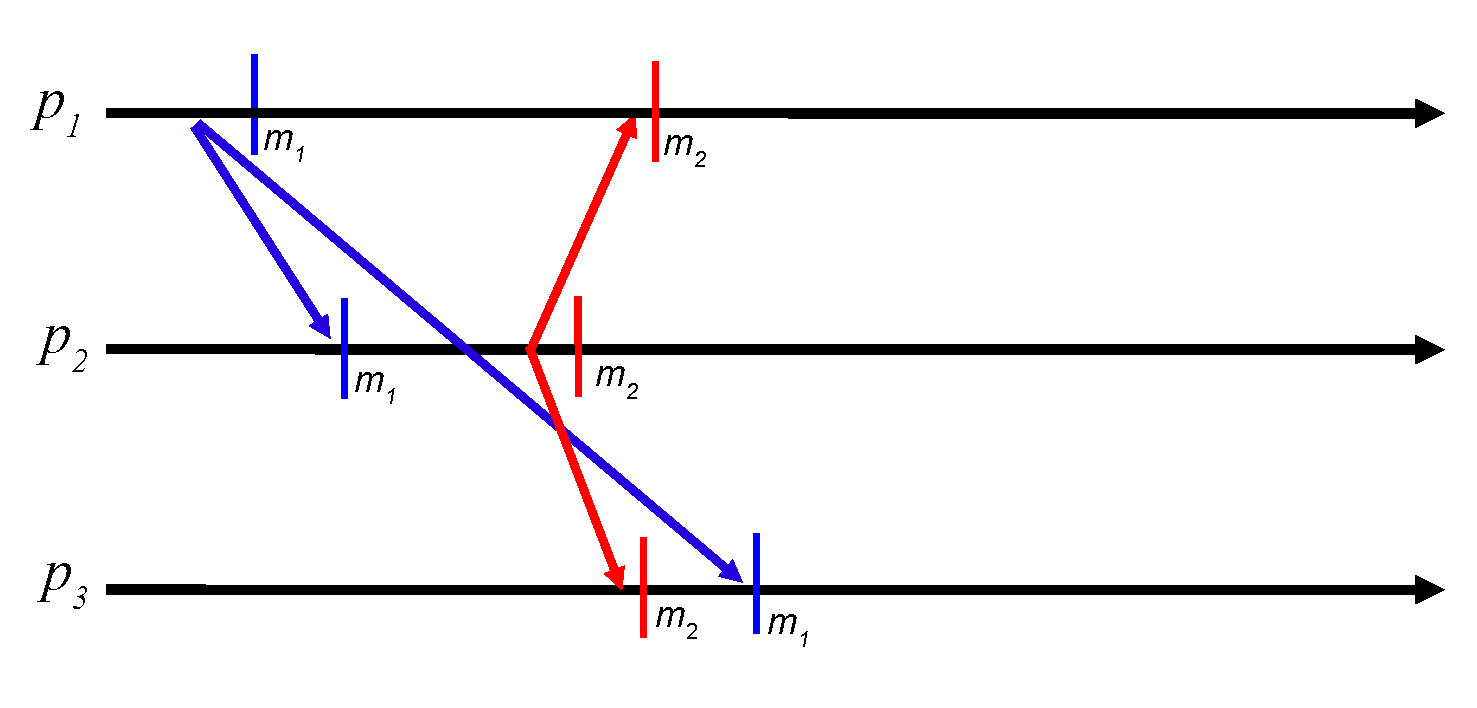
\includegraphics[width=0.8\textwidth]{figs/04/rb-causal2}
\end{figure}
		
\end{frame}

\begin{frame}

\begin{definition}[Causal Order]
If the broadcast of a message $m$ \alert{happens-before} the broadcast of a message $m'$, then 
no correct process delivers $m'$ unless it has previously delivered $m$
\[
  \broadcast_p(m) \rightarrow \broadcast_q(m') \Rightarrow \deliver_r(m) \rightarrow \deliver_r(m')
\]
\end{definition}

\structure{Is this causal?} \only<2>{Yes!}

\begin{figure}
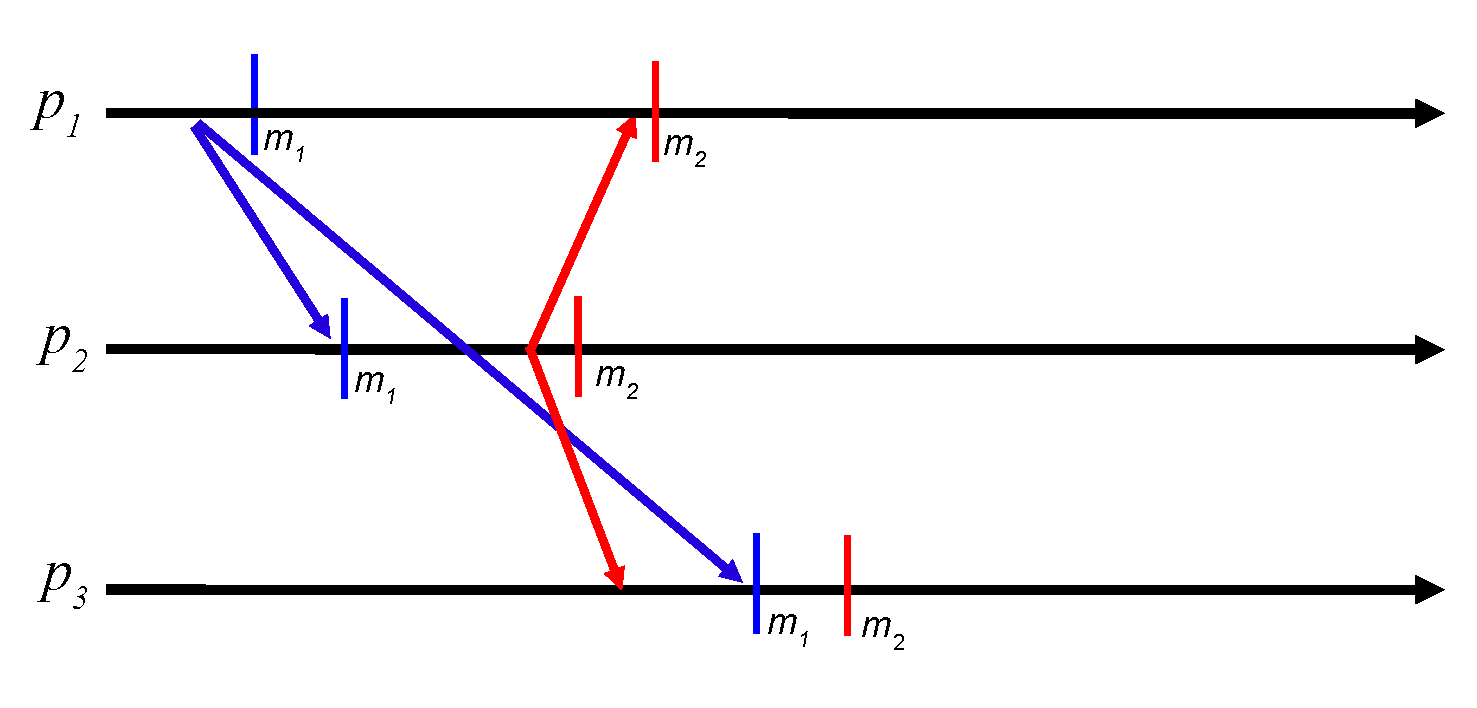
\includegraphics[width=0.8\textwidth]{figs/04/rb-causal3}
\end{figure}
		
\end{frame}

\begin{frame}

\begin{definition}[Causal Order]
If the broadcast of a message $m$ \alert{happens-before} the broadcast of a message $m'$, then 
no correct process delivers $m'$ unless it has previously delivered $m$
\[
  \broadcast_p(m) \rightarrow \broadcast_q(m') \Rightarrow \deliver_r(m) \rightarrow \deliver_r(m')
\]
\end{definition}

\structure{Is this causal?} \only<2>{Yes!}

\begin{figure}
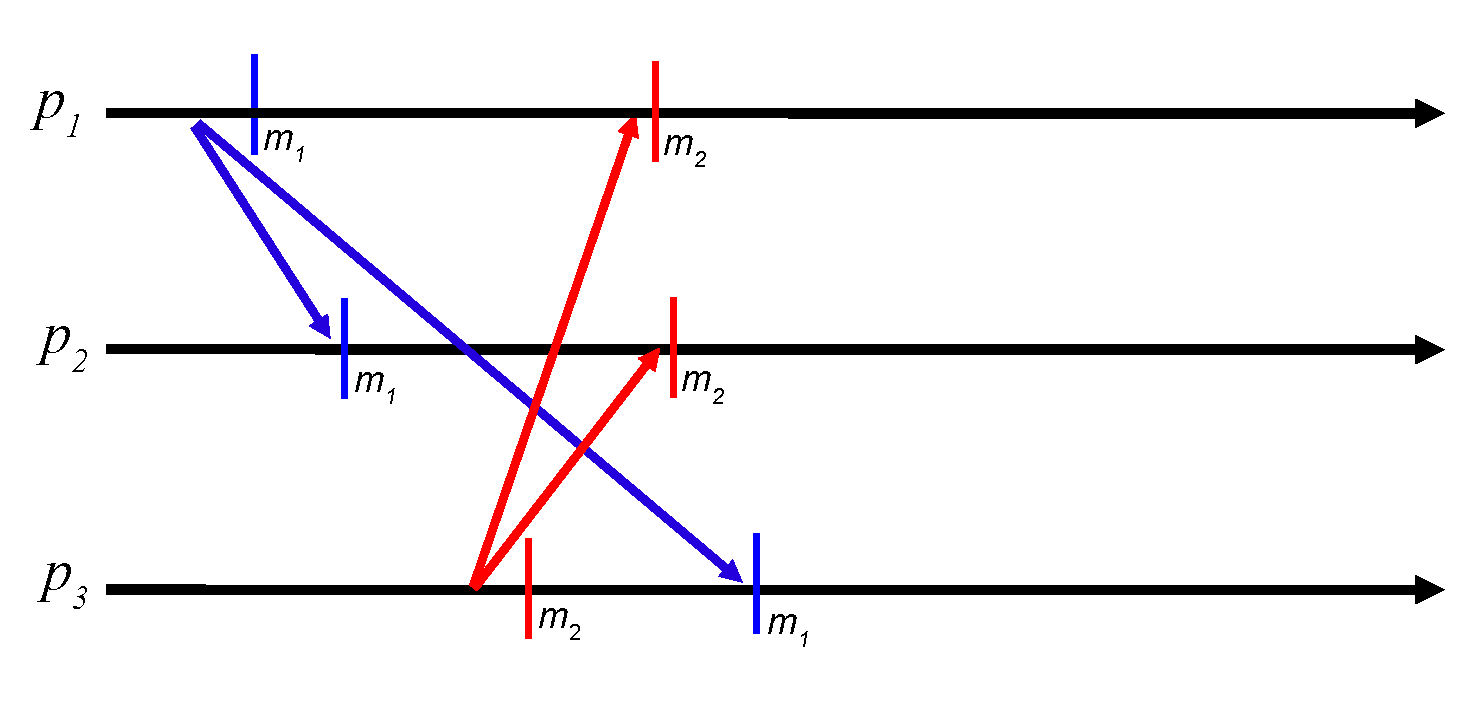
\includegraphics[width=0.8\textwidth]{figs/04/rb-causal1}
\end{figure}
		
\end{frame}

\begin{frame}{Message ordering}
\begin{block}{Problem}
Causal Broadcast does not impose any order on messages not causally related
\end{block}
\begin{example}
\BI
\item Consider a replicated database with two copies of a bank account
\item Initially, $\mathit{account} = 1000\$$
\item A user deposits 150\$ triggering a broadcast of $m_1 = \{ \textrm{add 150\$ to \emph{account}} \}$  
\item At the same time the bank initiates a broadcast of $m_2 = \{ \textrm{add 2\% interest to \emph{account}} \}$
\item Causal Broadcast allows two processes to deliver these updates in different order, creating inconsistency
\EI
\end{example}
\end{frame}


\begin{frame}

\begin{definition}[Total Order]
If correct processes $p$ and $q$ both deliver messages $m$,$m'$, then $p$ delivers $m$ before $m'$ if and only if $q$ delivers $m$ before $m'$
\[
  \deliver_p(m) \rightarrow \deliver_p(m') \Rightarrow \deliver_q(m) \rightarrow \deliver_q(m')
\]
\end{definition}

\structure{Is this totally ordered?} \only<2>{No!}

\begin{figure}
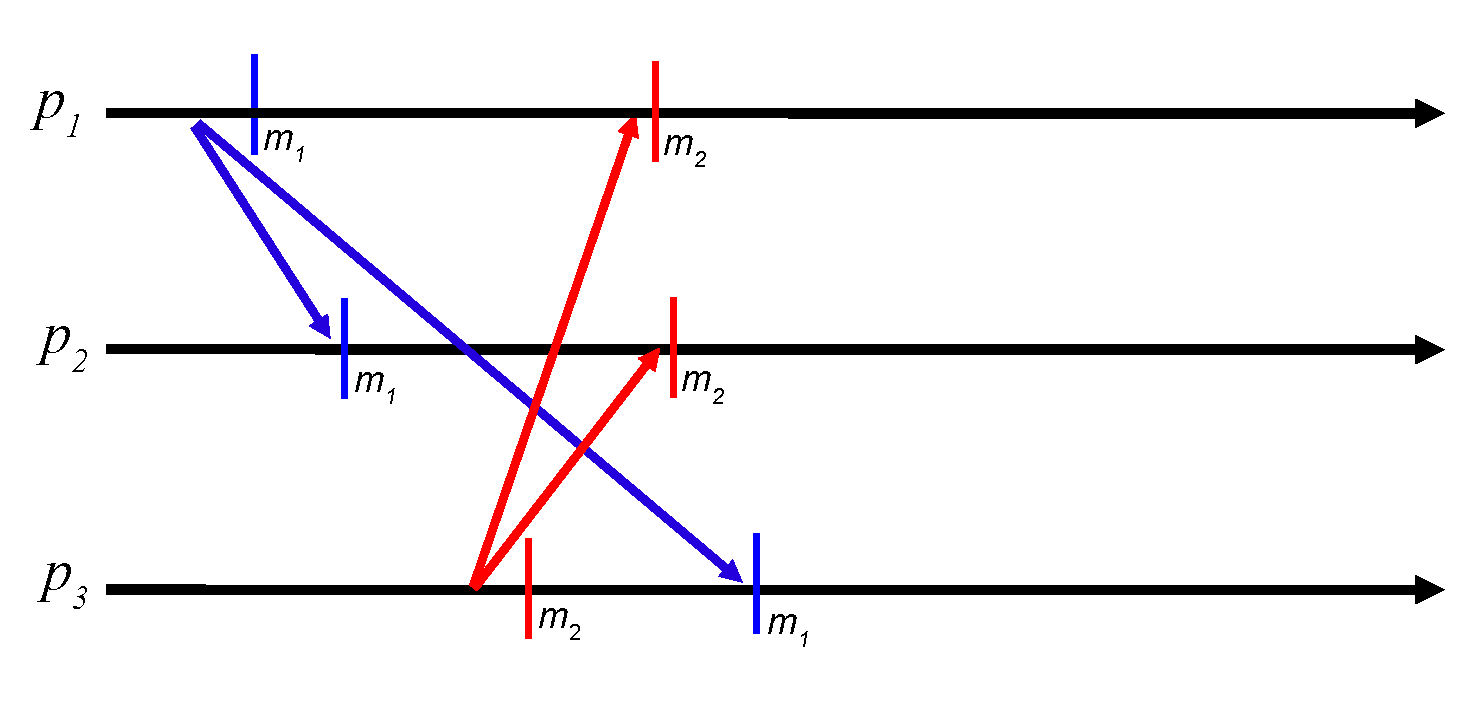
\includegraphics[width=0.8\textwidth]{figs/04/rb-causal1}
\end{figure}

\end{frame}

\begin{frame}

\begin{definition}[Total Order]
If correct processes $p$ and $q$ both deliver messages $m$,$m'$, then $p$ delivers $m$ before $m'$ if and only if $q$ delivers $m$ before $m'$
\[
  \deliver_p(m) \rightarrow \deliver_p(m') \Rightarrow \deliver_q(m) \rightarrow \deliver_q(m')
\]
\end{definition}

\structure{Is this totally ordered?} \only<2>{Yes!}

\begin{figure}
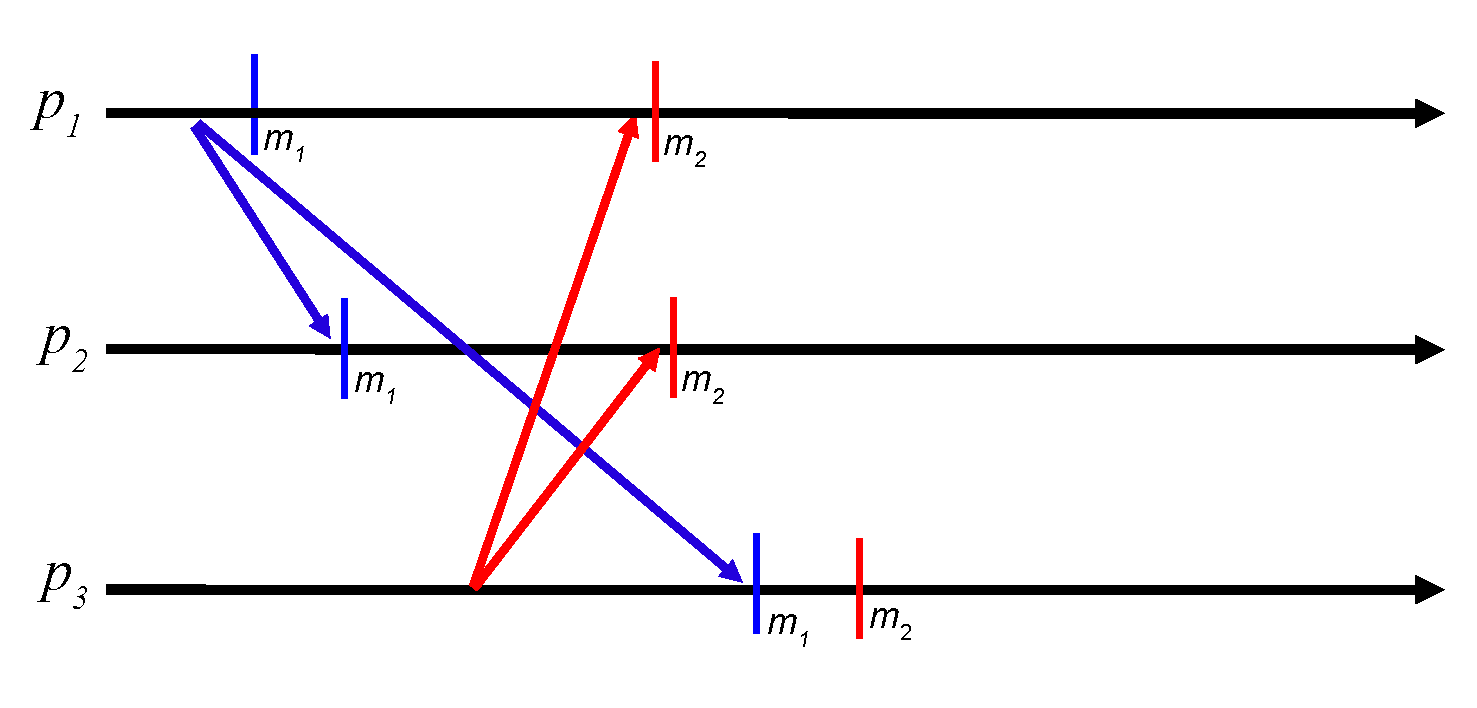
\includegraphics[width=0.8\textwidth]{figs/04/rb-total}
\end{figure}

\end{frame}

\begin{frame}{Uniform Versions}

{\footnotesize
\begin{definition}[Uniform FIFO Order]
If a process $p$ broadcasts a message $m$ before it broadcast a message $m'$, then 
no \sout{correct} process delivers $m'$ unless it has previously delivered $m$
\[
  \broadcast_p(m) \rightarrow \broadcast_p(m') \Rightarrow \deliver_q(m) \rightarrow \deliver_q(m')
\]
\end{definition}

\begin{definition}[Uniform Causal Order]
If the broadcast of a message $m$ \alert{happens-before} the broadcast of a message $m'$, then 
no \sout{correct} process delivers $m'$ unless it has previously delivered $m$
\[
  \broadcast_p(m) \rightarrow \broadcast_q(m') \Rightarrow \deliver_r(m) \rightarrow \deliver_r(m')
\]
\end{definition}

\begin{definition}[Uniform Total Order]
If \sout{correct} processes $p$ and $q$ both deliver messages $m$,$m'$, then $p$ delivers $m$ before $m'$ if and only if $q$ delivers $m$ before $m'$
\[
  \deliver_p(m) \rightarrow \deliver_p(m') \Rightarrow \deliver_q(m) \rightarrow \deliver_q(m')
\]
\end{definition}
}
\end{frame}

\subsection{A modular approach}

\begin{frame}{A modular approach to Broadcast}

\begin{figure}
	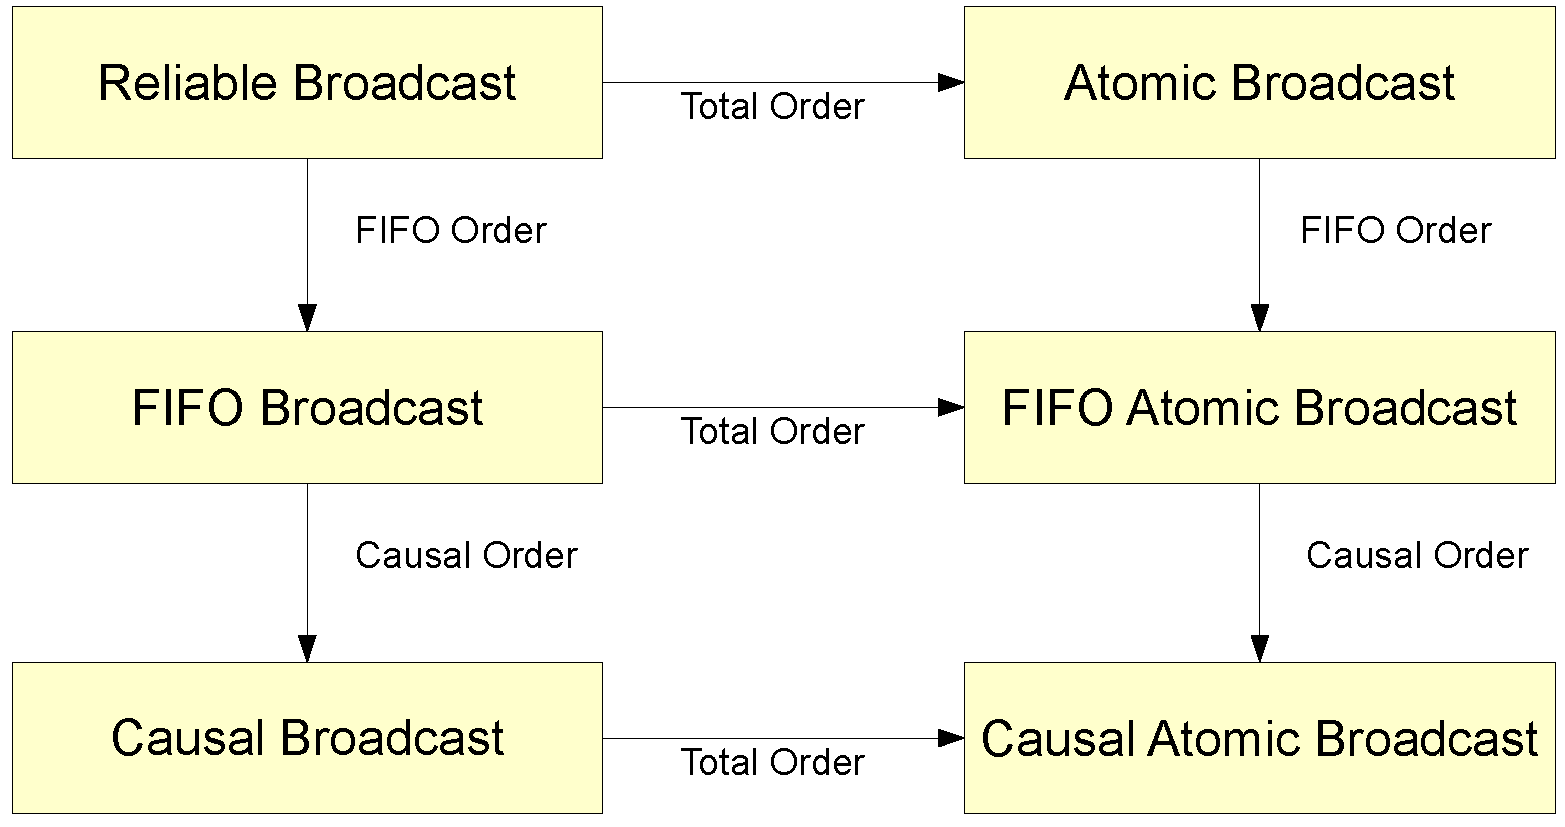
\includegraphics[width=\textwidth]{figs/04/rb-modular-rb1}
\end{figure}

\end{frame}

\begin{frame}{A modular approach to Broadcast}

\begin{figure}
	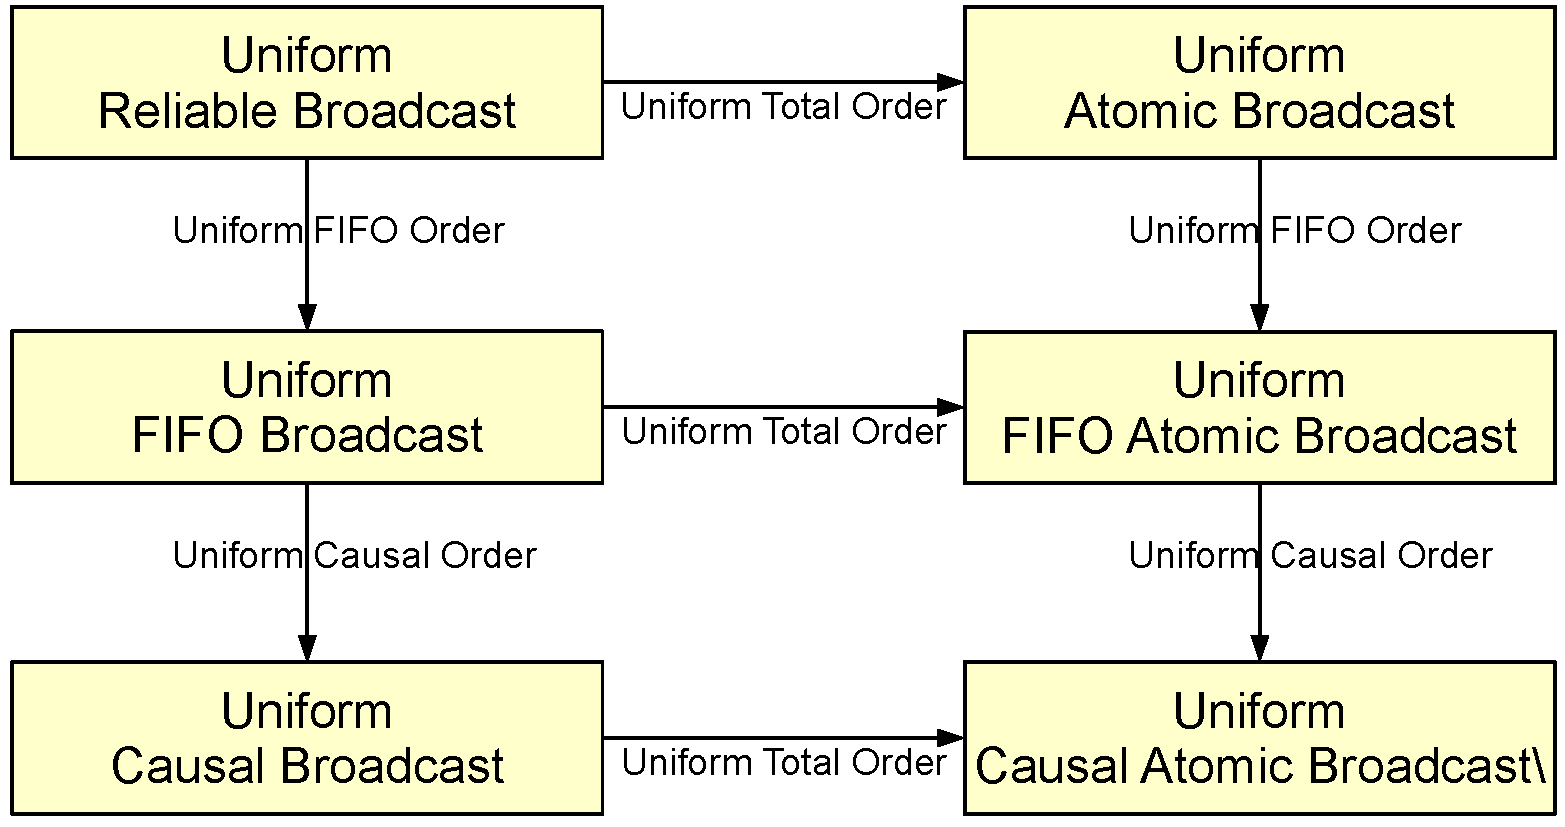
\includegraphics[width=\textwidth]{figs/04/rb-modular-urb1}
\end{figure}

\end{frame}



\begin{frame}{Transformation}
	
\begin{block}{Informal definition}
A broadcast transformation is an algorithm that takes a weaker broadcast 
algorithm and transform it into a stronger version
\end{block}

\begin{definition}[Transformation]
A \alert{transformation} from problem $A$ to problem $B$ is an algorithm $T_{A \rightarrow B}$ that converts 
any algorithm $A$ that solves problem $A$ into an algorithm $B$ that
solves problem $B$
\end{definition}

\begin{definition}[Preservation]
A transformation $T_{A \rightarrow B}$ \alert{preserves} property $P$ if it
converts any algorithm for $A$ into an algorithm that solves problem $B$ and
also satisfies $P$
\end{definition}
	
\end{frame}

\begin{frame}{Transformation}
\BIL
\item Properties of weakest RB must be preserved
  \BI
  \item \alert{Uniform Integrity}: preserved in all transformations
  \BI
    \item No message is created
    \item Messages are tagged to avoid re-delivery
  \EI
  \item \alert{Validity}, \alert{(Uniform) Agreement}: 
  \BI
    \item To be proved case by case
  \EI
  \EI
\item  To add Total Order:
  \BI
  \item We cannot start from a simple reliable broadcast
  \item We need stronger assumptions
  \EI
\EIL
\end{frame}

\begin{frame}{Transformation}
	
\begin{definition}[Blocking transformation]
A transformation of one broadcast algorithm into another is \alert{blocking}
if the resulting broadcast algorithm has a run in which a process delays the
delivery of a message for a later time.
\end{definition}

\begin{example}
FIFO Order
\end{example}

\end{frame}

\subsection{Algorithms and proofs}

\begin{frame}[shrink=12]{FIFO Order -- Algorithm}

\begin{Procedure}
\caption{FIFO Order Transformation executed by process $p$}

\UPON{initialization}{
  $\Set\ \Undelivered \gets \emptyset$\;
  $\INTEGER[\,]\ \Next \gets \NEW\ \INTEGER[1 \ldots |\Pi|]$\;
  \lForEach{$q \in \Pi$}{$\Next[q] \gets 1$\;}
}
\BlankLine
\UPON{$\fbroadcast(m)$}{
  $\rbroadcast(m)$\;
}
\BlankLine
\UPON{$\rdeliver(m)$}{
  $\Undelivered \gets \Undelivered \cup \{ m \}$\;
  \While{$\exists m' \in \Undelivered: \Sender(m') = \Sender(m)$ \AND\\ \qquad\qquad $\Seqn(m') = \Next[q]$}{
    $\fdeliver(m')$\;
    $\Next[q] \gets \Next[q]+1$\;
    $\Undelivered \gets \Undelivered - \{ m' \}$\;
  }
}
\end{Procedure}

\end{frame}

\begin{frame}{FIFO Order -- Proof}

\begin{theorem}
For any process $p$, if $\Next_p[q]=k$ then $p$ has F-delivered the first $k-1$ messages F-broadcast by $q$
\end{theorem}

\begin{theorem}
Suppose a correct process $p$ R-delivers a message $m$ from $q$ and F-delivers all the messages that $q$ F-broadcast before $m$. Then $p$ also F-delivers $m$
\end{theorem}

\BIL
\item \alert{Validity}, \alert{(Uniform) Agreement}, \alert{(Uniform) Total Order} are preserved
\item \alert{Uniform FIFO Order} is satisfied
\item The transformation is blocking
\EIL

\note{\footnotesize
\structure{Claim 2 -- Proof}
If $m'$ is the last message delivered from $\Sender(m)$, let $k$ be equal to $\Seqn(m')$. By claim 1, 
$\Next_p[q]=k+1$ and by definition, $\Seqn(m)=k+1$. Thus $m$ will be delivered as the next message.

\structure{Validity -- Proof}
\BI 
\item To F-broadcast $m$, a correct process $p$ R-broadcasts it.
\item It will eventually R-deliver $m$ (Validity of RB)
\item Suppose $m$ is the first message $p$ R-delivers, but not F-delivers
For claim 2, it will eventually F-deliver $m$. Absurd.
\EI

\structure{Uniform FIFO Order -- Proof}
\BI
\item Suppose a process $p$ F-delivers a message $m$ F-broadcast by $q$.
\item Let $\Seqn(m) = k$.
\item By the algorithm, just before F-delivering $m$, $\Next_p[q] = k$.
\item By Claim 1, $p$ has already F-delivered all the $k-1$ messages that
  $q$ F-broadcast before $m$, as wanted.
\EI
}

\end{frame}

\begin{frame}{Causal Order - Algorithm}

\structure{Two transformations}:

\BIL
\item Both based on FIFO Reliable Broadcast
\item One is non-blocking
  \BI
  \item Each message is tagged with “recent history”
  \item When a message is F-delivered, all the causal messages that have been F-delivered are locally delivered
  \item Does this recall anything?
  \EI
\item One blocking 
  \BI
  \item Based on vector clocks
  \EI
\EIL
\end{frame}

\begin{frame}[shrink=5]{Causal Order - Algorithm 1}

\begin{Procedure}
\caption{Causal Order Transformation executed by process $p$}

\UPON{initialization}{
  $\Set\ \Delivered \gets \emptyset$\Comment*[f]{Messages already C-delivered}\;
  $\Sequence\ \Recent \gets \langle \rangle$\Comment*[f]{Messages C-delivered since last C-broadcast}\;
}
\BlankLine
\UPON{$\cbroadcast(m)$}{
  $\fbroadcast(\Recent || m)$\;
  $\Recent \gets \langle \rangle$\;
}
\UPON{$\fdeliver(\langle m_1, \ldots, m_k \rangle)$}{
  \For{$i \gets 1$ \TO $k$}{
    \If{\NOT $m_i \notin \Delivered$}{
      $\Delivered \gets \Delivered \cup \{ m_i \}$\;
      $\Recent \gets \Recent || m_i$\;
      $\cdeliver(m_i)$\;
    }
  }
}

\end{Procedure}

\end{frame}

\begin{frame}{Causal Order - Algorithm 1}
	
\begin{figure}
	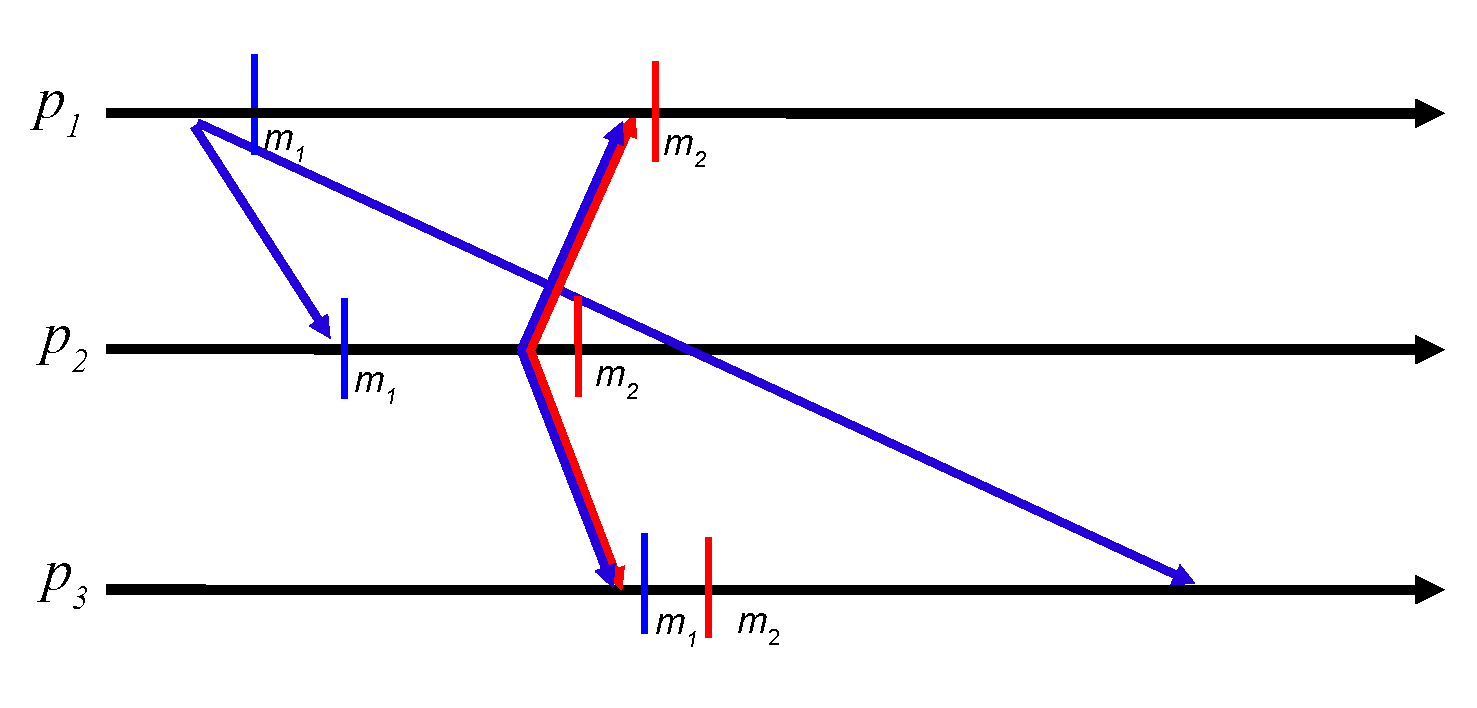
\includegraphics[width=\textwidth]{figs/04/rb-crb}
\end{figure}

\end{frame}

\begin{frame}{Causal Order -- Proof}

\BIL
\item \alert{Validity}, \alert{(Uniform) Agreement}, \alert{(Uniform) Total Order} are preserved
\item \alert{Uniform Causal Order} is satisfied
\item The transformation is non-blocking
\EIL

\end{frame}


\begin{frame}[shrink]{Causal Order - Algorithm 2}

\begin{Procedure}
\caption{Causal Order Transformation executed by process $p$}

\UPON{initialization}{
  $\Set\ \Undelivered \gets \emptyset$\Comment*[f]{Messages to be delivered}\;
  $\INTEGER[\,]\ \VC \gets \{ 0, \ldots, 0 \}$\Comment*[f]{Vector clock}\;
}
\BlankLine
\UPON{$\cbroadcast(m)$}{
  $\fbroadcast(\langle m, \VC \rangle)$\;
}
\UPON{$\fdeliver(\langle m, \TS \rangle)$}{
  $\Undelivered \gets \Undelivered \cup \{ \langle m, \TS \rangle \rangle$\;
  \While{$\exists \langle m', \TS' \rangle \in \Undelivered : \mbox{$\VC[\Sender(m')] = \TS'[\Sender(m')]-1$} \wedge 
    \mbox{\qquad\qquad $\forall s \neq \Sender(m'): \VC[s] \geq TS'[s]$}$}{
    $\cdeliver(m')$\;
    update $\VC$\;
    $\Undelivered \gets \Undelivered - \{ m \}$\;
  }
}
\end{Procedure}

\end{frame}

\begin{frame}{Causal Order - Algorithm 2}
	
\begin{figure}
	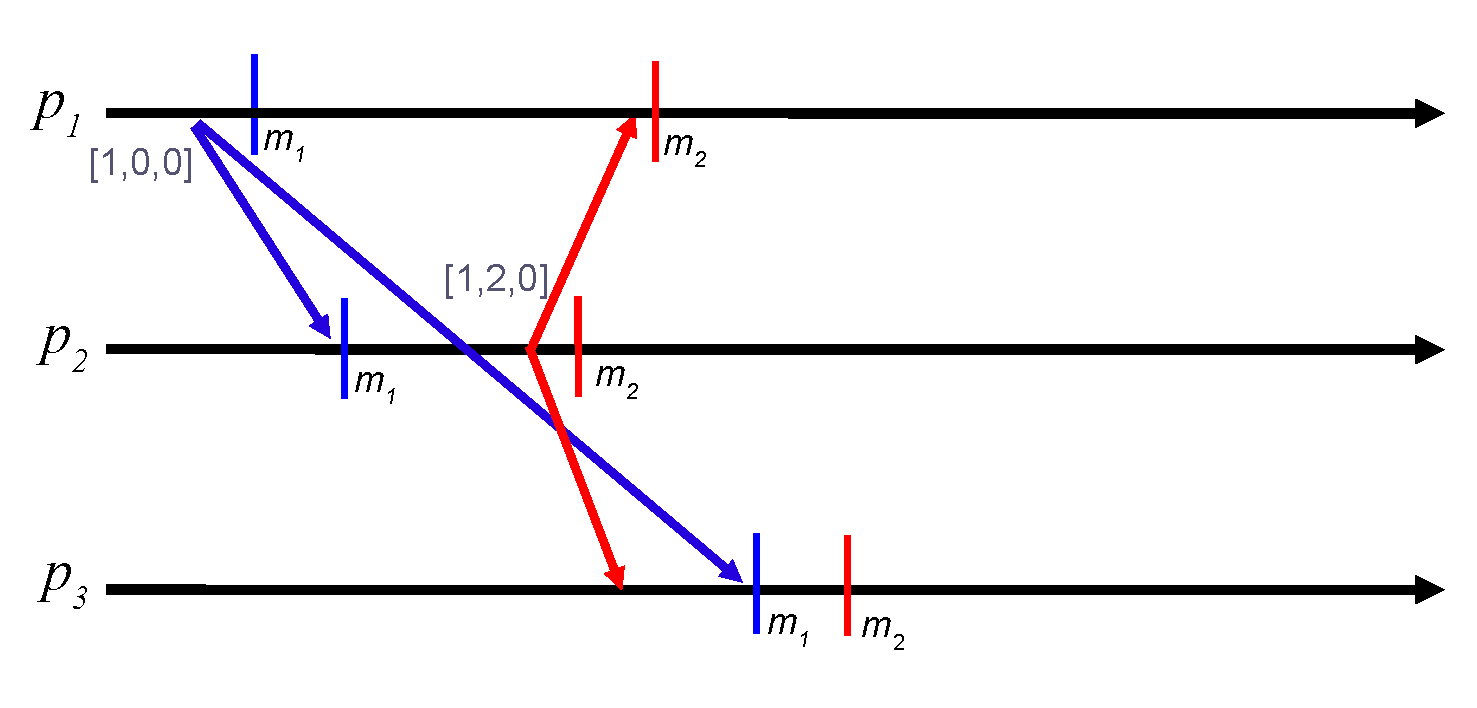
\includegraphics[width=\textwidth]{figs/04/rb-causal-vc}
\end{figure}

\end{frame}

\begin{frame}{Causal Order -- Proof}

\BIL
\item \alert{Validity}, \alert{(Uniform) Agreement}, \alert{(Uniform) Total Order} are preserved
\item \alert{Uniform Causal Order} is satisfied
\item The transformation is blocking
\EIL

\end{frame}


\begin{frame}{A modular approach to Broadcast}

\begin{figure}
	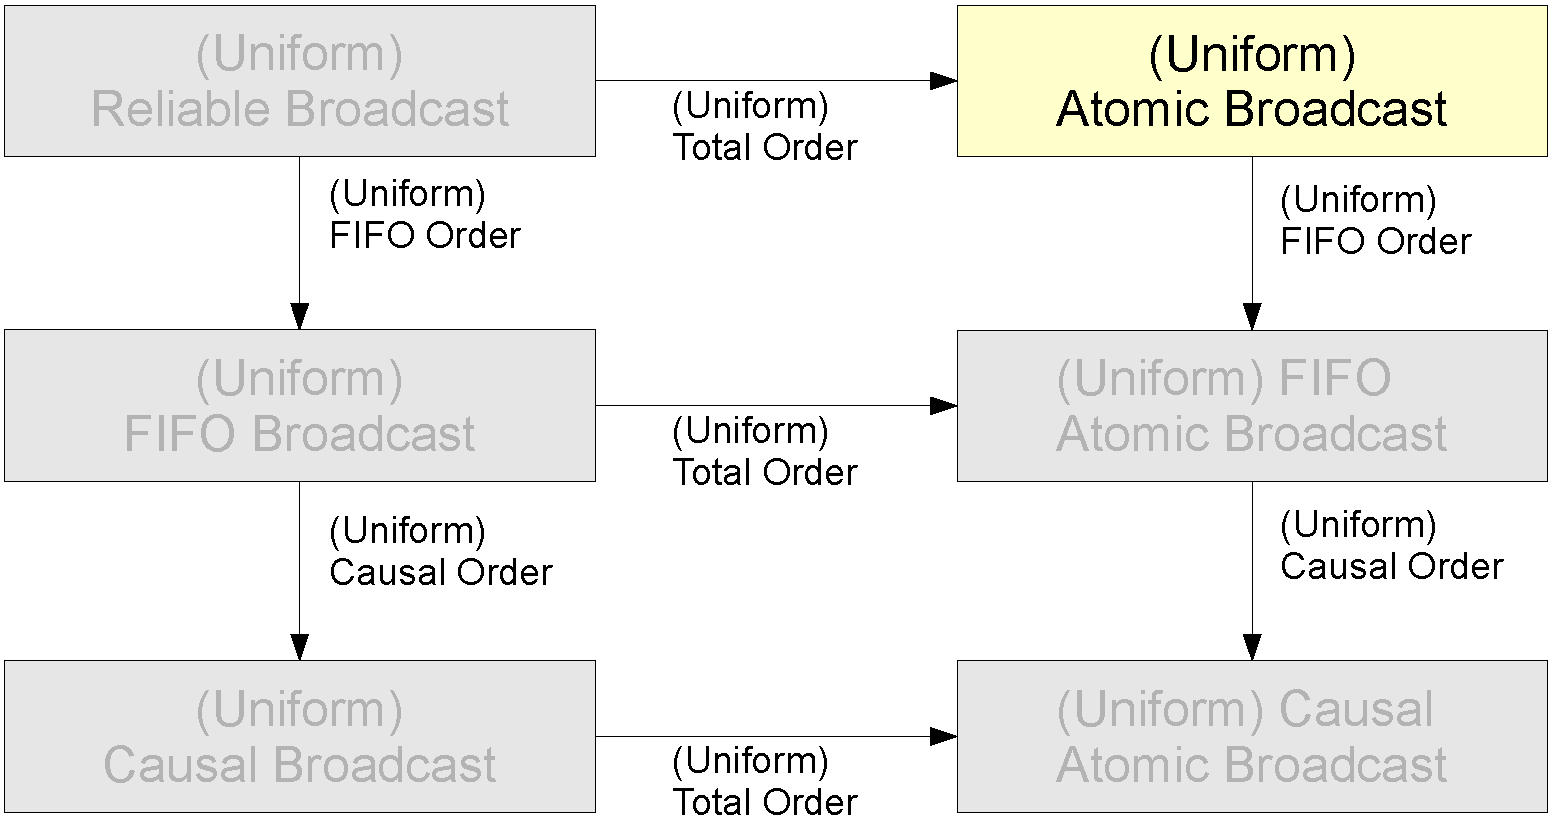
\includegraphics[width=\textwidth]{figs/04/rb-modular-summary}
\end{figure}

\end{frame}

\subsection{Atomic Broadcast}

\begin{frame}{Atomic Broadcast}
	
\structure{There are three approaches:}

\BEL
\item We add synchronous assumptions to our system
\item  We show that the Atomic Broadcast problem is \alert{equivalent} to the Consensus problem
\BI
\item There is an algorithm $T_{\mathit{Consensus} \rightarrow \mathit{Atomic Broadcast}}$
\item There is an algorithm $T_{\mathit{Atomic Broadcast} \rightarrow \mathit{Consensus}}$
\EI
\item Through a coordinator  (actual implementation, see later in group communication)
\EEL

\end{frame}


\begin{frame}{Timed Reliable Broadcast}

	
\begin{definition}[(Uniform) Real-Time $\Delta$-Timeliness]
There is a known constant $\Delta$ such that if a message $m$ is broadcast at real-time $t$, then no correct (any) process delivers $m$ after 
real-time $t+\Delta$
\end{definition}

\medskip
\begin{definition}[(Uniform) Local-Time $\Delta$-Timeliness]
There is a known constant $\Delta$ such that no correct (any) process delivers $m$ after local time $\TS(m)+\Delta$ on $p$'s clock,
where $\TS(m)$ is the timestamp obtained by the local clock of the sender
\end{definition}

\medskip
\begin{block}{Note}
(Uniform) Real-Time $\Delta$-Timeliness $\Rightarrow$\\ (Uniform) Local-Time $\Delta$-Timeliness
\end{block}
	
\end{frame}

\begin{frame}{Atomic Broadcast, Algorithm 1}
	
\begin{Procedure}
\caption{Total Order Transformation executed by process $p$}

\UPON{$\abroadcast(m)$}{
  $\tbroadcast(m)$\;
}
\BlankLine
\UPON{$\tdeliver(m)$}{
  \textbf{schedule} $\adeliver(m)$ \textbf{at time} $\TS(m) + \Delta$\;
}
\end{Procedure}
	
\end{frame}

\begin{frame}{Consensus}
	
\begin{columns}
	
\begin{column}{0.45\textwidth}
In the \alert{(Uniform) Consensus} problem, the processes \alert{propose}
values and need to \alert{decide} (agree) on one of these values
\begin{figure}
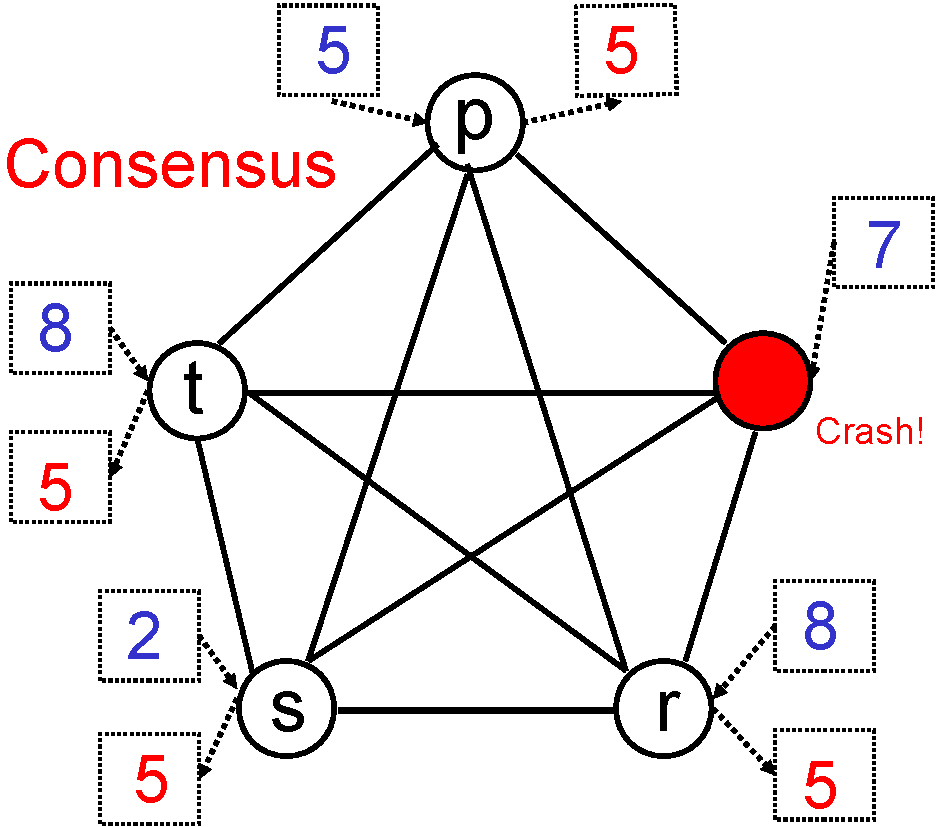
\includegraphics[width=\textwidth]{figs/04/rb-consensus}
\end{figure}

\end{column}

\begin{column}{0.55\textwidth}
\begin{definition}[Uniform Validity]
Any value decided is a value proposed
\end{definition} 
\begin{definition}[(Uniform) Agreement]
No two correct (any) processes decide differently 
\end{definition} 
\begin{definition}[Termination]
Every correct process eventually decides
\end{definition} 
\begin{definition}[Uniform Integrity]
Every process decides at most once
\end{definition} 
\end{column}
\end{columns}

	
\end{frame}

\begin{frame}{From Atomic Broadcast to Consensus}
	
\begin{Procedure}
\caption{Transformation executed by process $p$}

\UPON{initialization}{
  $\BOOLEAN\ \Decided \gets \FALSE$\;
}
\BlankLine
\UPON{$\Propose(v)$}{
  $\abroadcast(v)$\;
}
\BlankLine
\UPON{$\adeliver(v)$}{
  \If{\NOT \Decided}{
    $\Decided \gets \TRUE$\;
    $\Decide(u)$\;
  }
}
\end{Procedure}

\end{frame}

\begin{frame}[shrink]{From Consensus to Atomic Broadcast}

\begin{Procedure}
\caption{Transformation executed by process $p$}

\UPON{initialization}{
  $\Set\ \Unordered \gets \emptyset$\Comment*[f]{Messages to be ordered}\;
  $\Set\ \Delivered \gets \emptyset$\Comment*[f]{Messages already delivered}\;
  $\BOOLEAN\ \Wait \gets \FALSE$\Comment*[f]{\TRUE when Consensus is running}\;
  $\INTEGER\ s \gets 1$\Comment*[f]{Consensus protocol identifier}\;
}
\BlankLine
\UPON{$\abroadcast(m)$}{
  $\rbroadcast(m)$\;
}
\BlankLine
\UPON{$\rdeliver(m)$}{
  \If{\NOT $m \in \Delivered$}{
    $\Unordered \gets \Unordered \cup \{ m \}$\;
  }
}
\end{Procedure}

\end{frame}

\begin{frame}[shrink]{From Consensus to Atomic Broadcast}

\begin{Procedure}
\caption{Transformation executed by process $p$}

\UPON{$\Decide_s(S)$}{
  $\Unordered \gets \Unordered - S$\;
  \ForEach{$m \in S$}{
     $\adeliver(m)$\Comment*[f]{In some deterministic order}\;
  }
  $\Delivered \gets \Delivered \cup S$\;
  $s \gets s+1$\;
  $\Wait \gets \FALSE$\;
}
\BlankLine
\UPON{$\Unordered \neq \emptyset$ \AND \NOT $\Wait$}{
  $\Wait \gets \TRUE$\;
  $\Propose_s(\Unordered)$\;
}
\end{Procedure}

\end{frame}

\begin{frame}{Conclusions}

\begin{block}{Summary}
Consensus and total order broadcast are equivalent problems in an asynchronous system with crashes and Perfect Channels

\BIL
\item Consensus can be obtained from total order broadcast
\item Total order broadcast can be obtained from Consensus
\EIL
\end{block}

\begin{block}{Problem}
But in this way, we have moved the problem from Atomic Broadcast to Consensus.\\
Next step: can we solve Consensus?
\end{block}
 
\end{frame}


%%%%%%%%%%%%%%%%%%%%%%%%%%%%%%%%%%%%%%%%%%%%%%%%%%%%%%%%%%%%%%%%%%%%%%%%

\nocite{hadzilacos94modular}
\ReadingMaterial

\end{document}